\chapter{Introductory concepts}


\begin{notation}

We will consider all complexes to be over a field
$\mathbb{K}$ that will either be 
 $\mathbb{Q}$,
 $\mathbb{R}$,
 or 
  $\mathbb{C}$.
Unless otherwise stated.
\end{notation}



\newcommand{\R}{\mathbb{R}}

\section{Ordered complex and canonical form}


\begin{definition}[$\R$-Filtered complex]
Let $\{C_k\}_{k=0}^{\infty}$ be a complex. 
A $\R$-filtration (sometimes we will simply say a filtration), on $\{C_k\}_{k=0}^{\infty}$ 
is an increasing sequence of real numbers, $\{r_i\}_{i=0}^n$
so that for each $r_i$ there as associated $F_{\leq r_i}C_k\subset C_k$ for every $k$
that satisfies:

$$
\{0\}\subset
F_{\leq r_0}C_k
\subset
F_{\leq r_k}C_k
\subset
\cdots
\subset
F_{\leq r_n}C_k
=
C_k
$$
\end{definition}

As we well see, there are a lot of natural circumstances on which a filtration might arise. For example, 
the singular chain comples of a CW-complex is naturally filtered by its skeleton.

There are more structures we can put on a complex:


\begin{remark}
A filtrated complex has a natural order on the generators compatible with the filtration.
%Furthermore, if this filtration increases the dimension of each chain group by dimension $1$ (or $0$) on
%each step, then there is natural correspondence between the filtration and the ordering.
\end{remark}

\begin{definition}[Complex with ordered generators]

Let $\{C_k\}_{k=0}^{\infty}$ be a filtered chain complex, with some basis $\{\e{j}{i}\}$.
Then we say that $\{C_k\}_{k=0}^{\infty}$ has ordered generators when we fix the order 
$\e{k}{i}<e{l}{j}$ if  $k=l$ and $i<j$.

Notice we do not compare generators that live on different chain groups.
\end{definition}




\begin{definition}[Canonical form]

Let $\{C_k\}_{k=0}^{\infty}$ be a chain complex, with some basis $\{\e{k}{i}\}$.
Then we say that $\{C_k\}_{k=0}^{\infty}$ is in canonical form if,

\begin{enumerate}
\item $\partial \e{k}{i}$
is either $0$ or another generator.

\item If $\partial \e{k}{i}=\partial \e{l}{i}\neq 0$,
then $\e{k}{i}= \e{l}{i}$.
\end{enumerate}

\end{definition}

\begin{remark}
\label{canonicalformsplit}
An equivalent formulation of the canonical form is that we can find a basis $S$ 
of $\{C_k\}_{k=0}^{\infty}$ so that $S$
can be separated into: 
\begin{enumerate}
\item $S_H$: Generators of the homology of the complex.

\item $S_{\text{birth}}$: Births, that is, elements whose boundary is $0$, but get killed in homology by an element of higher degree.

\item $S_{\text{death}}$: Deaths, elements whose boundary is another generator. 

\item $\partial$ is a bijection between $S_{\text{death}}$ 
and $S_{\text{birth}}$.
\end{enumerate}

That is:

$$
S=S_{\text{birth}}\sqcup
S_{\text{death}}\sqcup
 S_H
$$ 
\end{remark}

\begin{theorem}
\cite{bar1994}
\label{canonicalform}
Every filtered chain complex can be reduced to 
one in canonical form by an upper-triangular change of basis
which preserves the filtration.

Furthermore, the canonical form is unique.
\end{theorem}

%\begin{prof}
First we prove that we prove the first statement. 
Let $\{C_k\}_{k=0}^\infty$ 
and a basis $\{\e{i}{j}\}_{i,j}$ 
with $\e{i}{j}\in C_i,\forall i$.

Let $i+1$ be the largest natural so that $C_{\geq n}$
is not in canonical form. Obviously, $i+1>0$, since $\partial | _{C_0}=0$.

Let $\e{i+1}{j}$ be the generator with smallest $j$ so that $\partial e^i_j$
is neither 0 nor another generator. Clearly, $i+j>0$, since $\partial | _{C_0}=0$.
	
Let $\partial \e{i+1}{j}=\sum \alpha_k \e{k}{j-1}$, then on the LHS, we have terms which are exact (that is, on $S_{\text{death}}$),
and those which are not. We move all the exact terms in the LHS of the form $\e{k}{j-1}=\partial \e{q}{j}$, with $q\leq i$.
$$
\partial\left(
\e{i+1}{j}
-
\sum_{q=1}^i
\e{j}{q}\alpha_{k(q)}
\right)
=
\sum \beta_k \e{k}{j-1}
$$

Here we separate two cases,
if the LHS is $0$, then we simply define 
$$
\f{j}{i+1}=
\e{i+1}{j}
-
\sum_{q=1}^i
\e{j}{q}\alpha_{k(q)}
$$

In this case, clearly the linear map $A \e{i+1}{j}=\f{i+1}{j}$ and the identity on the rest 
has an upper triangular matrix and $\partial \f{i+1}{j}=0$.

In the case we can find $\beta_{k_0}\neq 0 $ we pick such $k_0$ so it is maximal. Then:

$$
\partial
\frac{1}{\beta_{k_0}}
\left(
\e{i+1}{j}
-
\sum_{q=1}^i
\e{j}{q}\alpha_{k(q)}
\right)
=
\e{k_0}{j-1}
+
\sum_{k<k_0} \frac{\beta_k}{\beta_{k_0}} \e{k}{j-1}
$$

In this case, we define:

$$
\f{i+1}{j}
=
\frac{1}{\beta_{k_0}}
\left(
\e{i+1}{j}
-
\sum_{q=1}^i
\e{q}{j}\alpha_{k(q)}
\right);
\quad
\f{k_{0}}{j-1}
=
\e{k_0}{j-1}
+
\sum_{k<k_0} \frac{\beta_k}{\beta_{k_0}} \e{k}{j-1}
$$

Then clearly $\partial \f{i+1}{j}=\f{k_0}{j-1}$ and the obvious change of variable has the desired form.
This violates our minimality condition, therefore the first statement is proved.

Now we prove the uniqueness part: Suppose we have two bases in canonical form
$\{\e{i}{j}\}$ and $\{\f{i}{j}\}$. Then choose $i$ and $j$ so that for all $p<j$ and any $m$
or $p=j$ and $m<i$ then $\e{i}{j}=\f{i}{j}$. 

We can find coefficients $\alpha_k$ and $\beta_k$ so that:

$$
\f{i}{j}
=
\sum_{k=1}^i \alpha_k \e{k}{j},
\quad
\partial \f{i}{j} = \f{l}{j-1}
=
\sum_{n=1}^l \beta_k \e{k}{j}
$$

Hence 
$$
\partial \e{i}{j}=
\sum_{n=1}^l
\e{n}{j-1}\frac{\beta_n}{\alpha_i}
-
\sum_{k=1}^l
\partial \e{k}{j-1}\frac{\alpha_k}{\alpha_i}
$$

This proves the uniqueness of the canonical form since: $\partial \e{i}{j}=\e{m}{j-1},m>l$ and 
$\e{m}{j-1}\neq \partial a_k^j, \forall k\neq i$
 
\end{prof}



%\begin{definition}[Equivalent complexes]
%
%Two filtered complexes,
%$\{
%C_*
%\}$
%y
%$\{
%D_*
%\}$
%
%are said to be equivalent if 
%there is an isomorphism 
%
%\end{definition}

\begin{corollary}
Two filtered complexes are equivalent
\ifff they have the same canonical form.
\end{corollary}


\begin{corollary}{Category of filtered complexes is semi-simple.}
That is, any filtered complex, (or one with an ordered basis) can be expressed as a direct sum of 
1 dimensional complexes with trivial differential and 2 dimensional complexes with trivial homology.
\end{corollary}

\begin{prof}
Because any complex can we brought to canonical form, we can find a basis of the complex in the form of Remark \ref{canonicalformsplit}.
Then $\text{Span}(S_H)$ splits as a sum of 1 dimensional complexes with trivial differential, since the differential is trivial on $S_H$.
Similarly, the birth and death pairs splits into 2 dimensional complexes with one generator killing the other in homology.

\end{prof}

\section{Augmented metric spaces}

\begin{definition}
Let $(X,d)$ be a metric space,
we say it is augmented if it comes equiped with a function 
$f:X\to\mathbb{R}$.

\end{definition}

We will say that an augmented metric space is injective if $f$ is.

We will be interested in the case where $X$ is finite.

\section{Persistence complexes}

\begin{definition}[Persistent complex]
A persistence complex is a sequence of vector spaces 
$\{V_i\}_{0\leq i \leq n}$ and maps $f_i:V_i\to V_{i+1}$. That is, a diagram
as follows:


$$
\begin{tikzcd}
V_0 \arrow[r,"f_0"]
& V_1 \arrow[r]
& \cdots\arrow[r,"f_{n-1}"]
& V_n
\end{tikzcd}
$$


We denote $f_i^j
=
f_j\circ\cdots f_{i+1}\circ f_i
$ whith $i<j$.
Persistence diagrams may be of arbitrary cardinal,
as long as the indexed is set is well-ordered.

But we shall only considered them when they are finite or countable.

We further define it's graded Betti number as:

$$
b_i^j
=\left\{
\begin{array}{l c c}
\dim(V_i) & \text{if} & i=j\\
\text{rank}(f_i^j) & \text{if} & i<j\\
0 & \text{if} & i>j\\
\end{array}
\right.
$$

\end{definition}

We give examples of useful persistence diagrams in \ref{examplespersistence}.

\begin{example}[Interval module]
We define the interval module for $i<j$
to be the module where all maps are either the trivial ones, 
being the identity whenever possible and the zero map otherwise and 
the $V_k$ to be:

$$
V_k
=
\left\{
\begin{array}{l l}
\mathbb{K} & \text{if } i\leq k\leq j\\
0 & \text{otherwise} 
\end{array}
\right.
$$


We denote it by $m(i,j)$.

\end{example}



\begin{proposition}\cite{zomcar2002}
The category of countable persistence complex is equivalent to the one of graded modules over
$\mathbb{K}[t]$
\end{proposition}

\begin{proposition}\cite{zomcar2002}
Finite persistence diagrams are classified by 
their graded Betti numbers.

\end{proposition}


\subsection{Representations of the persistent complexes}

%\begin{definition}[Ranks diagrams]
%Given a persistence diagram, it's rank diagram
%is a subset of ${(x,y)\in[0,1]^2,x\leq y}$
%
%\end{definition}


\begin{definition}[Persistence diagrams]

\end{definition}

%\begin{definition}[Persistence diagrams]
%
%We call a persistence diagram to a finite family of half lines, indexed by $0,1,...$
%so that there is a discrete collection of points on each line and there are segments connecting points
%on a line of index $i$ to a line of index $i-1$.
%
%Furthermore, this segments always connect point of higher value with points of lower value.
%\end{definition}



Usually we can represent persistence modules as diagrams,
as is illustrated by the following example.
%We clarify this definition with an example:

\begin{example}
The diagram below is a persistence diagram, notice that we can recover the original module in a natural 
way:

\begin{enumerate}


\item To the line of index $k$ we assign
it the complex $C_k$.

\item Assign a generator to every point on every line a generator of $C_k$

\item We define the differential operator $\partial$
in the following way. If there is no segment coming out of the point, we define its differential to be zero.
If two points are joined by a line, we define the differential of one as the other.

\end{enumerate}

For example, in this particular case the associated complex would be:

\begin{enumerate}

\item $C_0 = \{\e{0}{0},\e{1}{0}\}$

\item $C_1 = \{\e{0}{1},\e{1}{1}\}$

\item $C_0 = \{\e{0}{2},\e{1}{2}\}$

\item $\partial \e{1}{1}=\e{0}{1}$, $\partial \e{0}{2}=\e{0}{1}$ and 
$0$ on the rest of the generators.
\end{enumerate}

And obviosuly $S_{\text{birth}}=\{
\e{0}{1},
\e{0}{1}
\}$,
$S_{\text{death}}=\{
\e{1}{1},
\e{0}{2}
\}$,
$
S_H=\{
\e{0}{0},
\e{1}{2}
\}
$

\end{example}

\begin{center}
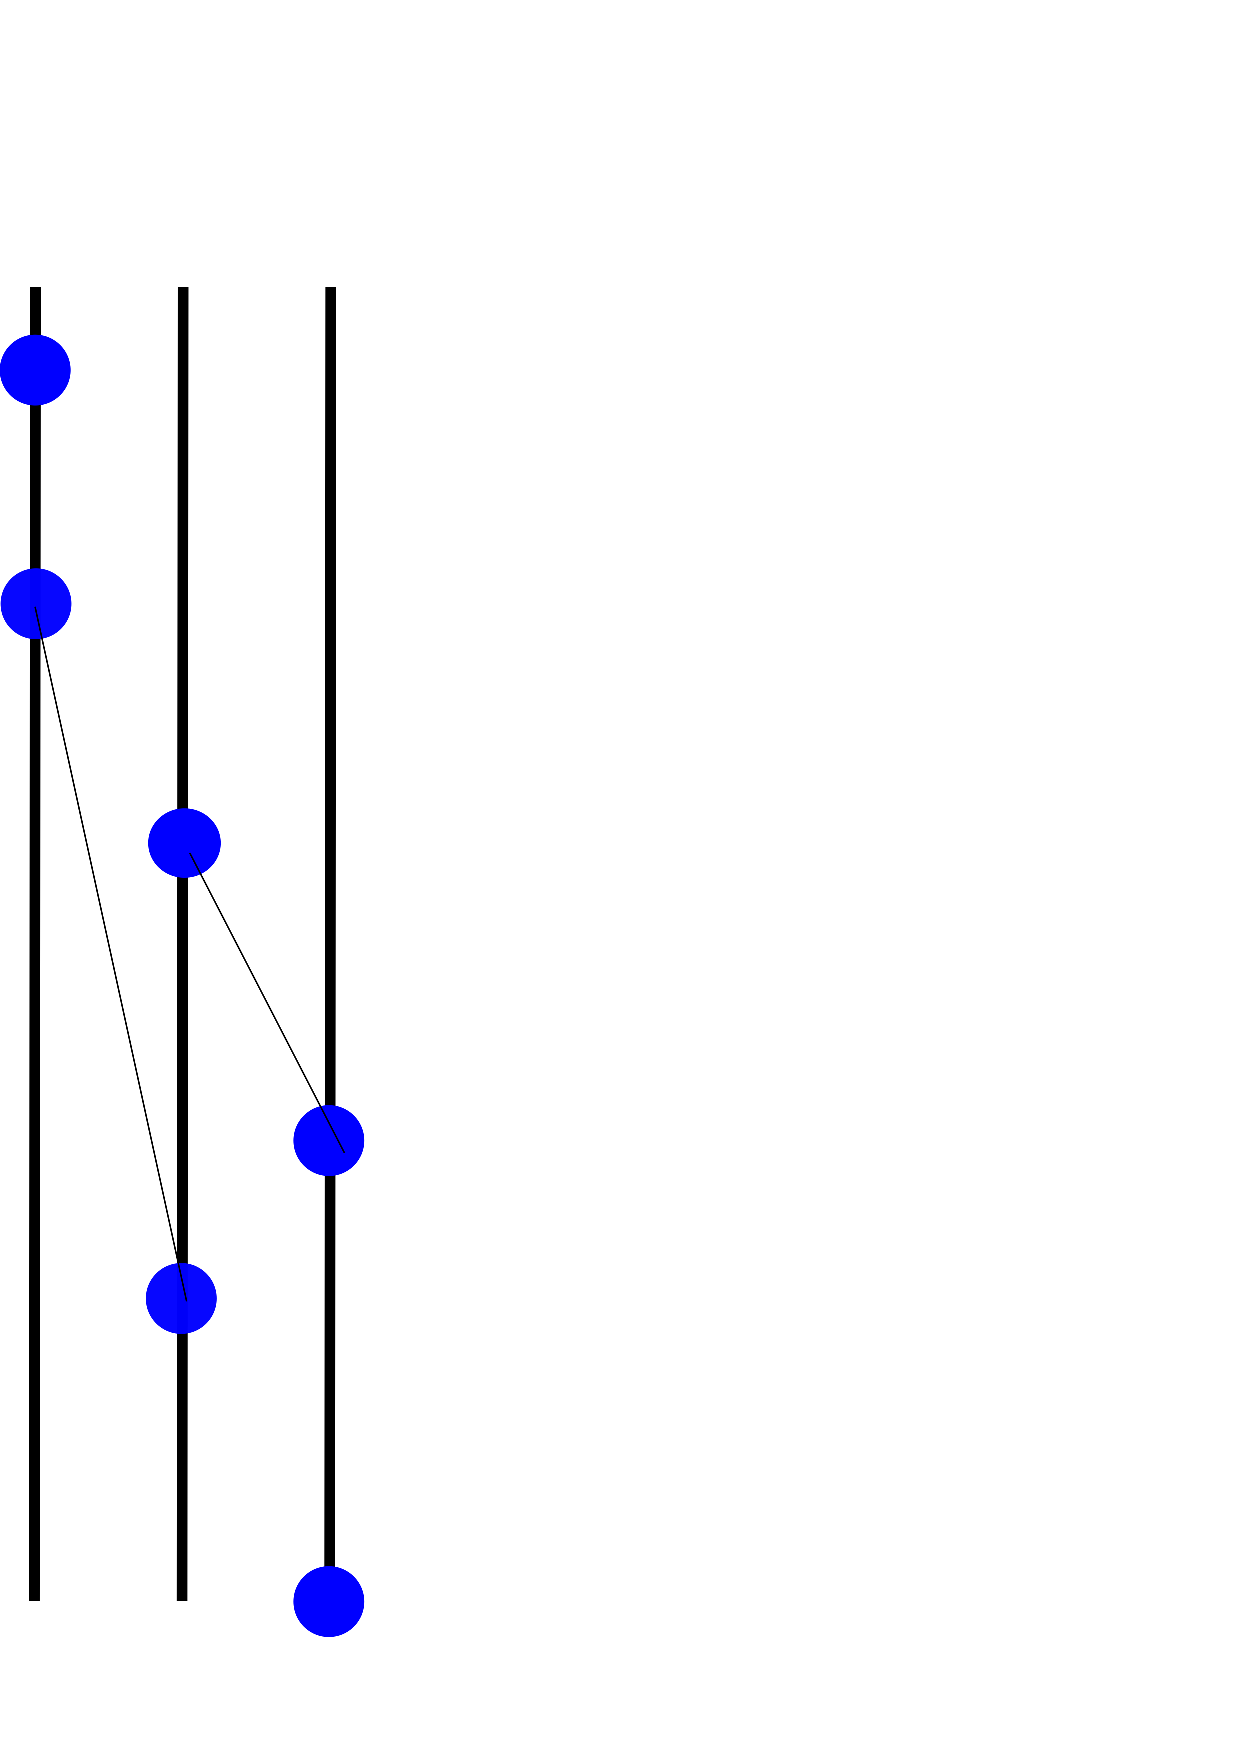
\includegraphics[height=4cm, width=4cm]{persistence_diagram1.png}
\end{center}


Clearly, from any complex in canonical form we can construct an associated persistent diagram by reversing the above process.
In the above example we ignored the filtration of the complex, but we consider that the diagram is filtered by height.
 Therefore:

\begin{proposition}[Canonical form = Persistence diagrams]

There is a natural equivalence between persistence diagrams and canonical forms.

\end{proposition}


Persistence diagrams are not the only way we can represent a canonical form. 
Another important example are codebars.

\begin{definition}
[Codebars]

By codebar we will mean a representation of similar to one below,
that a collection of bars, each one index (although index might be repeated),
where finite bars represent births and deaths and infinite bars represent elements that generate the homology of the complex.
\end{definition}

\begin{example}
This example represents the barcode
associated to the complex of the previous example.
\end{example}

\begin{center}
\includegraphics[height=4cm,width=7cm]{barcode1.png}
\end{center}


\subsection{Some important examples of persistent complexes}
\label{examplespersistence}

\begin{definition}[Discrete morse complex]
Let $f:M\to\mathbb{R}$ be a morse function from a compact manifold 
with finitely many critical points $t_0<\cdots<t_n$. Then the following diagram
is a persistence complex:

$$
\begin{tikzcd}
H^{dR}(f^{-1}(-\infty,t_0)) \arrow[r,"\subseteq"]
& H^{dR}(f^{-1}(-\infty,t_1)) \arrow[r,"\subseteq"]
& \cdots\arrow[r,"\subseteq"]
& H^{dR}(f^{-1}(-\infty,t_n))
\end{tikzcd}
$$

Where $H^{dR}$ is the de Rham complex and $\subseteq$
is homomorphism induced by the natural inclusion.

\end{definition}

\begin{definition}[{\Cech} Complex]

Let $X\subset \R^n$ be a discrete subset. Then, for $d>0$, we define the {\Cech}
complex of level $\epsilon$ as the following simplicial set:

%$$
%X_d 
%=
%\{
%x\in\R^n:
%d(x,X)\leq d
%\} 
%$$

$$
\tilde{C}_\epsilon(X)
=
\{
\sigma \subset X :
\bigcap_{y\in\sigma} B(y,\epsilon)\neq \emptyset
\}
$$

The {\Cech} complex is defined as $\{\tilde{C}_\epsilon\}_{\epsilon>0}$

\end{definition}

However, in practice the {\Cech} complex can get too large to handle, notice that when $\epsilon$ is large enough,
the {\Cech} complex equals the power set of $X$. One solution to this is using the 
Vietories-Rips complex.



\begin{definition}[Vietoris-Rips Complex]
Let $X\subset \R^n$ be a discrete subset. Then, for $d>0$, we define the \Cech
complex of level $\epsilon$ as the following simplicial set:

$$
\tilde{R}_\epsilon(X)
=
\{
\sigma \subset X :
\text{diam}(\sigma)\leq \epsilon
\}
$$

\end{definition}

The Vietoris-Rips complex is defined as $\{\tilde{R}_\epsilon\}_{\epsilon>0}$.

\begin{remark}
Notice than if both the {\Cech} and Vietories-Rips complex, the complex grows in a discrete manner meaning
that there are only finitely many $\epsilon$ values for which the complex changes if $\epsilon$ is pertubed slightly.

Furthermore, this complex are naturally filtrated and thus, they can be brought into canonical form.
\end{remark}

There are many softwares that can be used to compute the
{\Cech} and Vietories-Rips complexes, most of them rely on bringing the complex to canonical form.


Another important example is the following:

\begin{definition}[Bifiltrated Vietories-Rips complex]

Let $\mathcal{X}=(X,d,f)$ be an augmented metric space,
let $X_\sigma=f^{-1}(-\infty,\sigma)$ we define the bifiltrated
Vietories-Rips complex as the complex
$\{\tilde{R}_\epsilon^\sigma\}_{\epsilon>0,\sigma}$
with:

$$
\tilde{R}_\epsilon^\sigma=
\tilde{R}_\epsilon(X_\sigma)
$$

\end{definition}

\section{Motivation}

Another way in which filtered complexes arise is through Morse functions. For example, let's 
consider the following manifold with the morse function being the height function:

%\subsection{Arnold's extension problem}

%\chapter{Canonical form=Persistence diagrams}



%\section{Optimal sequence of metamorphoses of the canonical form}
%
%One natural question for quickly computing the canonical form of a complex is 
%the following: What is the shortest way to bring a complex to canonical form only using 
%relatively simple transformations.
%Now, what do we mean by simple transformations?
%
%\begin{definition}
%We say that a transformation of a complex is simple if it is one of the following:
%
%\begin{itemize}[label={}]
%
%\item {\bf Type (1)}: 
%A transformation sending $b$ to $b\pm a$
%
%\item {\bf Type (2)}:
%A transformation sending $b$ to $b\pm a$
%
%\end{itemize}
%
%
%\end{definition}


\section{Example of canonical form}

The proof of theorem \ref{canonicalform} gives an
algorithmic way to bring a complex into canonical form, 
we now expose how this methods works with an example. 
The general case should be clear afterwards.



